\documentclass{beamer}
\usetheme{metropolis}
\usepackage{graphicx}
\usepackage{subfig}
\usepackage{tcolorbox}
\title{Calculus-Based Physics-2: Electricity, Magnetism, and Thermodynamics (PHYS180-02): Unit 2}
\author{Jordan Hanson}
\institute{Whittier College Department of Physics and Astronomy}

\begin{document}
\maketitle

\section{Unit 1 Review}

\begin{frame}{Unit 1 Summary}
\textbf{Reading: Chapters 1 and 2}
\begin{enumerate}
\item Temperature, Heat, and the 0th Law of Thermodynamics
\item Heat flow and transfer mechanisms
\item Kinetic Theory of Gases
\end{enumerate}
\end{frame}

\begin{frame}{Unit 1 Review Problems}
\small
James Prescott Joule first published in December 1840, an abstract in the Proceedings of the Royal Society, suggesting that heat could be generated by an electrical current. Joule immersed a length of wire in a fixed mass of water and measured the temperature rise due to a known current flowing through the wire for a 30 minute period. By varying the current and the length of the wire he deduced that the heat produced was proportional to the square of the current multiplied by the electrical resistance of the immersed wire. \\ \vspace{0.5cm} Wikipedia: \url{https://en.wikipedia.org/wiki/Joule_heating}.
\end{frame}

\begin{frame}{Unit 1 Review Problems}
Suppose the wire of J. Joule is carrying 50 W of power.  If the mass of the water in the container is 1 kg, how long will it take to raise the temperature of the water by 5 degrees?  (The heat capacity of water is 4186 J/kg/$^{\circ}$C).
\begin{itemize}
\item A: 10 seconds
\item B: 80 seconds
\item C: 420 seconds
\item D: 3600 seconds
\end{itemize}
\end{frame}

\begin{frame}{Unit 1 Review Problems}
Suppose the the water begins at 95 $^{\circ}$C, and ends at 100 $^{\circ}$C.  How long will it take to boil away all of the water?  (The latent heat of vaporization of water is 2256 kJ/kg).
\begin{itemize}
\item A: Less than a minute
\item B: Several minutes
\item C: About an hour
\item D: Several hours
\end{itemize}
\end{frame}

\begin{frame}{Unit 1 Review Problems}
\begin{figure}
\centering
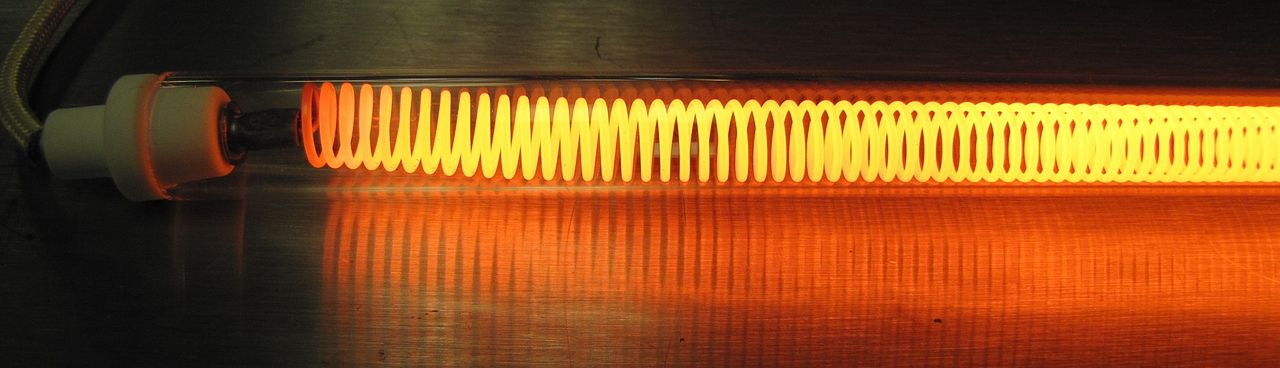
\includegraphics[width=0.9\textwidth]{figures/toaster.JPG}
\caption{\label{fig:toast} An example of Joule heating in a toaster coupling.}
\end{figure}
\end{frame}

\section{Summary}

\begin{frame}{Unit 2 Summary}
\textbf{Reading: Chapters 3 and 4}
\begin{enumerate}
\item The First Law of Thermodynamics
\item The Second Law of Thermodynamics
\end{enumerate}
\end{frame}

\section{JITT Reading -  1.3}

\begin{frame}{JITT Reading -  1.3}
\begin{enumerate}
\item In your own words, why is the internal energy path-independent, for paths on a p-V diagram?
\item If a system gains heat but the internal energy does not change, according to the first law of thermodynamics, what should happen?
\item What is the difference between absolute error and fractional error?
\end{enumerate}
\end{frame}

\begin{frame}{JITT Reading -  1.3}
\small
In your own words, why is the internal energy path-independent, for paths on a p-V diagram? \\ \hrulefill \\
``It doesn’t matter how you go from place one place to the next.'' \\
``The internal energy path is independent for paths on the p-V diagram because internal energy is only dependent on temperature, not on pressure and volume.'' \\
``Internal energy is path independent because none of the atoms touch each other and the potential energy is constant.''
\end{frame}

\begin{frame}{JITT Reading -  1.3}
\small
If a system gains heat but the internal energy does not change, according to the first law of thermodynamics, what should happen? \\ \hrulefill \\
``According to the first law of thermodynamics, the system would have to do work in some way, usually by moving a piston which would increase the volume of the system.'' \\
``If a system gains heat but the internal energy doesn't change, according to the first law of thermodynamics work is lost.''
\end{frame}

\begin{frame}{JITT Reading -  1.3}
\small
What is the difference between absolute error and fractional error? \\ \hrulefill \\
\textit{(Some people expressed confusion, so we will do some examples).} \\ \vspace{0.5cm}
\begin{columns}[T]
\begin{column}{0.5\textwidth}
\centering
\underline{Absolute error:} Let $x$ and $y$ be quantities we are measuring, and let $z=x-y$.
\begin{align}
x\pm\sigma_x & \\
y\pm\sigma_y & \\
\end{align}
The quantities $\sigma_x$, $\sigma_y$, and $\sigma_z$ are called \textit{absolute errors,} and they have the same units $x$, $y$, and $z$.
\end{column}
\vline \hspace{0.1cm}
\begin{column}{0.5\textwidth}
\centering
\underline{Fractional error:} Let $x$ and $y$ be quantities we are measuring, and let $z=xy$.
\begin{align}
x\pm\sigma_x & \\
y\pm\sigma_y & \\
\frac{\sigma_z}{z} &= \sqrt{\left(\frac{\sigma_x}{x}\right)^2 + \left(\frac{\sigma_y}{y}\right)^2} 
\end{align}
The quantities $\sigma_x/x$, $\sigma_y/y$, and $\sigma_z/z$ are called \textit{fractional errors,} and they have the no units.
\end{column}
\end{columns}
\end{frame}

\begin{frame}{JITT Reading -  1.3}
To summarize, three rules:
\begin{enumerate}
\item Adding or subtracting variables with absolute errors: absolute errors combine \textit{in quadrature}.
\item Multiplying or dividing variables with absolute errors: fractional errors combine \textit{in quadrature}.
\item Multiplying a variable with absolute errors by a constant: the constant just multiplies the absolute error.
\end{enumerate}
\end{frame}

\begin{frame}{Fractional versus Absolute Error}
Supose a thermodynamic system has $Q = 100\pm 10$ kJ of heat \textit{added to it}, and $W = 100\pm 10$ kJ of work \textit{done on it.}  What is the change in internal energy, accounting for absolute errors?
\end{frame}

\begin{frame}{Fractional versus Absolute Error}
Suppose we measure the temperature $T=200$ K of an ideal gas, with some absolute error $\sigma_T = \pm 50$ K.  Suppose we measure the number of moles $n=2.0$ in the gas with some absolute error $\sigma_n = \pm 0.5$.  What is the internal energy $E_{int}$ of the ideal gas?
\end{frame}

\begin{frame}{Fractional versus Absolute Error}
A block of frozen substance has a measured mass of $4.0\pm 1.0$ kg, and a measured latent heat of $100\pm 25$ kJ/kg.  How much heat (within errors) is required to melt it?
\end{frame}

\section{The First Law of Thermodynamics}

\begin{frame}{The First Law of Thermodynamics}
\alert{Equation of state}: The equation of state of a system, in general, looks like this:
\begin{equation}
f(p,V,T) = 0
\end{equation}
\begin{itemize}
\item $V$ is an \textbf{extensive} variable.
\item $p$ and $T$ are \textbf{intensive} variables.
\item Holding \textit{intensive} variables constant, doubling the mass of a system doubles the volume.  That is the relationship between intensive and extensive variables.
\end{itemize}
\end{frame}

\begin{frame}{The First Law of Thermodynamics}
\alert{The equation of state of an ideal gas} looks like this:
\begin{equation}
pV - nRT = 0
\end{equation}
Which of the following is correct?
\begin{itemize}
\item A: The extensive variables are $p$, $V$, and $R$
\item B: The extensive variables are $n$ and $V$, and $p$, and $T$ are the intensive ones
\item C: The only extensive variable is $n$, and $p$ is the only intensive one
\item D: There are no extensive variables because none of them is mass
\end{itemize}
\end{frame}

\begin{frame}{The First Law of Thermodynamics}
Recall that the definition of work done on a system is:
\begin{equation}
W = \int \vec{F} \cdot d\vec{x}
\label{eq:work}
\end{equation}
\begin{itemize}
\item $\vec{F}$ is the net force acting on the system
\item $d\vec{x}$ is the incremental displacement
\end{itemize}
\end{frame}

\begin{frame}{The First Law of Thermodynamics}
Example: suppose the force is gravity, near the surface of the Earth $\vec{F} = -mg \hat{y}$, and an object at height $h$ is released.
\begin{equation}
W = \int \vec{F} \cdot d\vec{x} = -mg \hat{y} \cdot -h\hat{y} = mgh
\label{eq:work2}
\end{equation}
\begin{itemize}
\item $\vec{F}$ is the net force acting on the system
\item $d\vec{x}$ is the incremental displacement
\item Work-energy theorem can give the final speed: $\frac{1}{2}mv_{\rm f}^2 = mgh$.
\end{itemize}
\end{frame}

\begin{frame}{The First Law of Thermodynamics}
Definition of work, applied to a thermodynamic system \textit{with an equation of state}:
\begin{equation}
W = \int \vec{F} \cdot d\vec{x} = \int p\vec{A} \cdot d\vec{x} = \int p dV
\label{eq:work3}
\end{equation}
\begin{itemize}
\item $\vec{A}$ and $d\vec{x}$ assumed to be parallel
\item $p$ is constant over $d\vec{x}$
\end{itemize}
\end{frame}

\begin{frame}{The First Law of Thermodynamics}
Definition of work, applied to a thermodynamic system \textit{with an equation of state}:
\begin{equation}
W = \int p dV
\label{eq:work4}
\end{equation}
\textbf{Group board exercise:} Substitute the Ideal Gas Law into Eq. \ref{eq:work4}, to derive the work done \textit{when temperature is constant and $V$ is the independent variable}. \\ \vspace{0.5cm}
\textit{Hint: the integral of $\frac{1}{x}$ is $\ln x + C$.} \\
\vspace{0.5cm}
\textbf{Group board exercise:} Repeat, but at \textit{constant pressure} instead of constant temperature, again with $V$ as the independent variable.
\end{frame}

\begin{frame}{The First Law of Thermodynamics}
The van der Waals \textit{equation of state} for one mole of gas is: 
\begin{equation}
\left(p+\frac{a}{V^2}\right)\left(V-b\right) - RT = 0
\label{eq:vanDerWaals}
\end{equation}
\textbf{Group board exercise:} Substitute this equation of state into Eq. \ref{eq:work4}, to find the work done by isothermal expansion.  Compare to the isothermal result from the Idea Gas Law, and recover the previous result for $W$ by setting $a$ and $b$ to zero.
\end{frame}

\begin{frame}{The First Law of Thermodynamics}
\begin{figure}
\centering
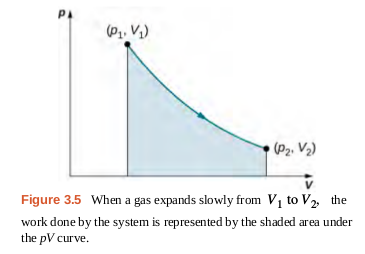
\includegraphics[width=0.45\textwidth]{figures/area1.png}
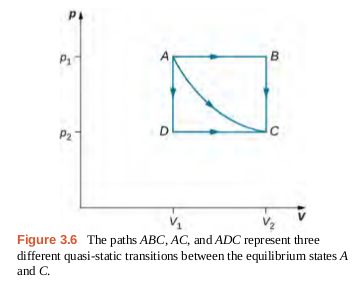
\includegraphics[width=0.45\textwidth]{figures/area2.png}
\caption{\label{fig:area} \small On a $pV$ diagram, work is the area under the curve, in the same fashion that it is the area under the curve on a force displacement diagram.}
\end{figure}
\end{frame}

\begin{frame}{The First Law of Thermodynamics}
The van der Waals \textit{equation of state} for $n$ moles of gas is: 
\begin{equation}
\left(p+a\left(\frac{n}{V}\right)^2\right)\left(V-nb\right) - nRT = 0
\label{eq:vanDerWaals2}
\end{equation}
\textbf{Show that the work done in an isothermal process is}: 
\begin{equation}
\boxed{
W = nRT\ln\left(\frac{V_f-nb}{V_i-nb}\right)-\frac{an^2}{V_iV_f}\Delta V}
\end{equation}
\end{frame}

\begin{frame}{The First Law of Thermodynamics}
Questions:
\begin{enumerate}
\item What is the \textit{fractional error} between idea work and actual work, accounting for intermolecular forces and molecular volume?
\item What is the meaning of $b$, physically?
\end{enumerate}
\textit{Reading: error analysis document on Moodle, and JITT 1.3 for Friday on reading it.}
\end{frame}

\begin{frame}{The First Law of Thermodynamics}
How much energy is available to do work, in the form of heat?  (For example, if we expand a gas at constant pressure, by how much can we decrease the temperature?) \\ \vspace{0.5cm}
Recall from the prior chapter that 
\begin{equation}
\boxed{
E_{\rm int} = \frac{3}{2}nRT = \frac{3}{2}nN_{\rm A}k_{\rm B}T = \frac{3}{2}NkT}
\label{eq:internal}
\end{equation}
The \textit{internal energy} of a gas must be comprised of the average kinetic energies of the molecules.  Here we ignore molecular interactions.
\end{frame}

\begin{frame}{The First Law of Thermodynamics}
\begin{tcolorbox}[colback=white,colframe=red!40!blue,title=The First Law of Thermodynamics]
\alert{Associated with every equilibrium state of a system is its internal energy $E_{\rm int}$.  The change in $E_{\rm int}$ for any transition between two equilibrium states is $\Delta E_{\rm int} = Q-W$, where $Q$ is the heat exchanged by the system and $W$ is the work done on or by the system.}
\end{tcolorbox}
\begin{itemize}
\item If heat is added to the system: $Q>0$
\item If heat is removed from the system: $Q<0$
\item If work is done by the system: $W>0$
\item If work is done on the system: $W<0$
\end{itemize}
\end{frame}

\begin{frame}{The First Law of Thermodynamics}
In each of the following scenarios, select the best answer:
\small
\begin{itemize}
\item A: $E_{\rm int}$ increases
\item B: $E_{\rm int}$ decreases
\item C: $E_{\rm int}$ does not change
\item D: I am confused.
\end{itemize}
\small
\begin{itemize}
\item Scenario 1: \alert{A gas expands against a piston, doing some work, but the gas loses no heat.}
\item Scenario 2: A gas expands against a piston, performing 10 J of work.  A separate device adds 10 J of heat to the gas.
\item Scenario 3: A piston is pushed against a gas, requiring 10 J of work.  A separate device adds 10 J of heat to the gas.
\end{itemize}
\end{frame}

\begin{frame}{The First Law of Thermodynamics}
In each of the following scenarios, select the best answer:
\small
\begin{itemize}
\item A: $E_{\rm int}$ increases
\item B: $E_{\rm int}$ decreases
\item C: $E_{\rm int}$ does not change
\item D: I am confused.
\end{itemize}
\small
\begin{itemize}
\item Scenario 1: A gas expands against a piston, doing some work, but the gas loses no heat.
\item Scenario 2: \alert{A gas expands against a piston, performing 10 J of work.  A separate device adds 10 J of heat to the gas.}
\item Scenario 3: A piston is pushed against a gas, requiring 10 J of work.  A separate device adds 10 J of heat to the gas.
\end{itemize}
\end{frame}

\begin{frame}{The First Law of Thermodynamics}
In each of the following scenarios, select the best answer:
\small
\begin{itemize}
\item A: $E_{\rm int}$ increases
\item B: $E_{\rm int}$ decreases
\item C: $E_{\rm int}$ does not change
\item D: I am confused.
\end{itemize}
\small
\begin{itemize}
\item Scenario 1: A gas expands against a piston, doing some work, but the gas loses no heat.
\item Scenario 2: A gas expands against a piston, performing 10 J of work.  A separate device adds 10 J of heat to the gas.
\item Scenario 3: \alert{A piston is pushed against a gas, requiring 10 J of work.  A separate device adds 10 J of heat to the gas.}
\end{itemize}
\end{frame}

\begin{frame}{The First Law of Thermodynamics}
In each of the following scenarios, select the best answer:
\small
\begin{itemize}
\item A: $E_{\rm int}$ increases
\item B: $E_{\rm int}$ decreases
\item C: $E_{\rm int}$ does not change
\item D: I am confused.
\end{itemize}
\small
\begin{itemize}
\item Scenario 4: \alert{A cold scientist clutches a warm canteen of water to his chest (the system is the canteen).}
\item Scenario 5: A cylinder of gas has a piston on one end.  Someone pulls the piston slowly, doing 10 J of work.
\end{itemize}
\end{frame}

\begin{frame}{The First Law of Thermodynamics}
In each of the following scenarios, select the best answer:
\small
\begin{itemize}
\item A: $E_{\rm int}$ increases
\item B: $E_{\rm int}$ decreases
\item C: $E_{\rm int}$ does not change
\item D: I am confused.
\end{itemize}
\small
\begin{itemize}
\item Scenario 4: A cold scientist clutches a warm canteen of water to his chest (the system is the canteen).
\item Scenario 5: \alert{A cylinder of gas has a piston on one end.  Someone pulls the piston slowly, doing 10 J of work.}
\end{itemize}
\end{frame}

\begin{frame}{The First Law of Thermodynamics}
\begin{figure}
\centering
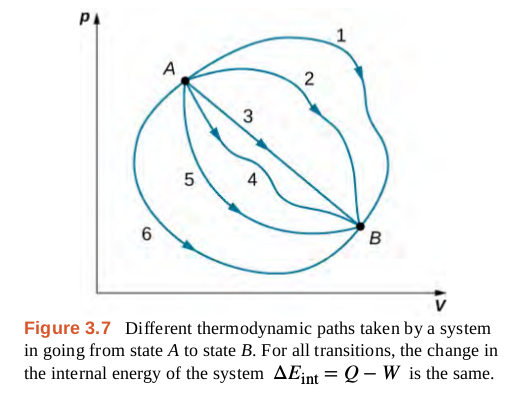
\includegraphics[width=0.6\textwidth]{figures/states1.png}
\caption{\label{fig:states} The internal energy for a given state depends only on the temperature, and not the path taken to arrive at that state.}
\end{figure}
\end{frame}

\begin{frame}{The First Law of Thermodynamics}
\small
\begin{columns}[T]
\begin{column}{0.5\textwidth}
\small Which of the following is true of the \textit{work done by the system}, for paths 2-5?
\begin{itemize}
\item A: Path 2 corresponds to the most work done, and path 5 the least work done.
\item B: Path 5 corresponds to the most work done, and path 2 the least work done.
\item C: Path 3 corresponds to the most work done, and path 4 the least work done.
\item D: Path 4 corresponds to the most work done, and path 3 the least work done.
\end{itemize}
\end{column}
\begin{column}{0.5\textwidth}
\begin{figure}
\centering
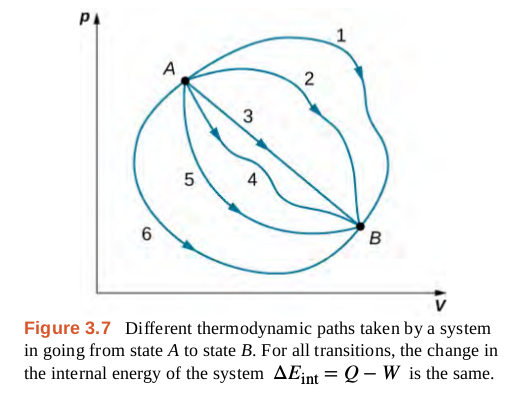
\includegraphics[width=\textwidth]{figures/states1.png}
\caption{\label{fig:states2} Use this diagram to answer the questions at left.}
\end{figure}
\end{column}
\end{columns}
\end{frame}

\begin{frame}{The First Law of Thermodynamics}
\begin{columns}[T]
\begin{column}{0.5\textwidth}
\small Suppose $\Delta E_{\rm int} = 0$.  Which path performs the most net work?
\begin{itemize}
\item A: AB: path 2, BA: returns along path 2
\item B: AB: path 2, BA: returns along path 3
\item C: AB: path 2, BA: returns along path 4
\item D: AB: path 2, BA: returns along path 5
\end{itemize}
\end{column}
\begin{column}{0.5\textwidth}
\begin{figure}
\centering
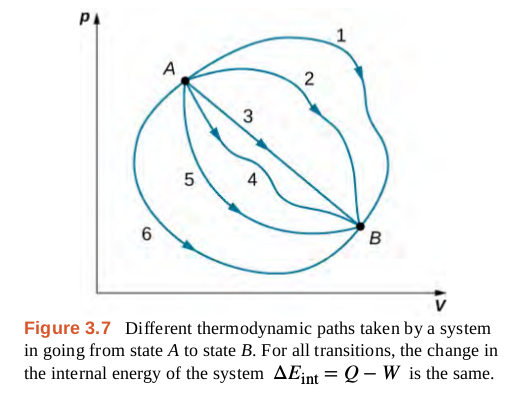
\includegraphics[width=\textwidth]{figures/states1.png}
\caption{\label{fig:states3} Use this diagram to answer the questions at left.}
\end{figure}
\end{column}
\end{columns}
\end{frame}

\begin{frame}{The First Law of Thermodynamics}
\begin{columns}[T]
\begin{column}{0.5\textwidth}
\small Suppose the system in question is an ideal gas.  Which path most likely represents a transition with constant temperature?
\begin{itemize}
\item A: Path 3
\item B: Path 2
\item C: Path 5
\item D: Path 1
\end{itemize}
\end{column}
\begin{column}{0.5\textwidth}
\begin{figure}
\centering
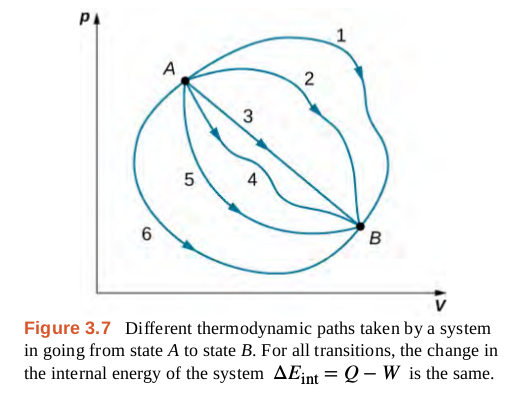
\includegraphics[width=\textwidth]{figures/states1.png}
\caption{\label{fig:states4} Use this diagram to answer the questions at left}
\end{figure}
\end{column}
\end{columns}
\end{frame}

\begin{frame}{The First Law of Thermodynamics}
Recall that the work done by an $n$ moles of an expanding ideal gas at constant temperature $T$ is given by $W = nRT\ln(V_{\rm f}/V_{\rm i})$, where $R = 8.314$ J/mole/Kelvin.  Calculate the work done if heat is added to 2 moles of an ideal gas at 300 K such that the volume of the gas grows by a factor of 2.
\begin{itemize}
\item A: 416 J
\item B: 520 J
\item C: 3460 J
\item D: 4320 J
\end{itemize} 
\end{frame}

\begin{frame}{The First Law of Thermodynamics}
Same scenario, but calculate the work if the gas was at a constant temperature of 200 K.
\begin{itemize}
\item A: 2305 J
\item B: 3410 J
\item C: 280 J
\item D: 320 J
\end{itemize} 
\end{frame}

\begin{frame}{The First Law of Thermodynamics}
If the temperature remains at 200K during the process, what is the heat transferred into or out of the system?
\begin{itemize}
\item A: -2305 J
\item B: 2305 J
\item C: -3410 J
\item D: 3410 J
\end{itemize} 
\end{frame}

\begin{frame}{The First Law of Thermodynamics}
Suppose we have a system where we can add external heat into a rocket, and then 100 percent of that heat is converted to kinetic energy for the rocket.  If the rocket has 0.1 kg of mass, and $g = 10$ m/s/s, how much heat is required to launch the rocket to a height of 50 meters?
\begin{itemize}
\item A: 20 J
\item B: 30 J
\item C: 40 J
\item D: 50 J
\end{itemize} 
\end{frame}

\begin{frame}{The First Law of Thermodynamics}
If in the heat-to-rocket system, we have to provide the heat first to 2 moles of an ideal gas, what would be the required temperature change?
\begin{itemize}
\item A: 2 degrees C
\item B: 3 degrees C
\item C: 20 degrees C
\item D: 30 degrees C
\end{itemize} 
\end{frame}

\begin{frame}{The First Law of Thermodynamics}
In the previous two problems we equated heat energy with mechanical energy: $mgh = Q$, and then calculated $Q$ with $Q=\frac{3}{2}nRT$.  Thus, we used $mgh = \frac{3}{2}nRT$.  Let's try one with kinetic energy instead of potential energy. \\ \vspace{0.5cm}
If we are using the heat stored in 2 moles of an ideal gas, what temperature change is required to get that heat to accelerate a 0.1 kg object to 10 m/s? \textit{Is the temperature change positive or negative?}
\begin{itemize}
\item A: 3 degrees C
\item B: 2 degrees C
\item C: 0.3 degrees C
\item D: 0.2 degrees C
\end{itemize} 
\end{frame}

\begin{frame}{The First Law of Thermodynamics}
\begin{figure}
\centering
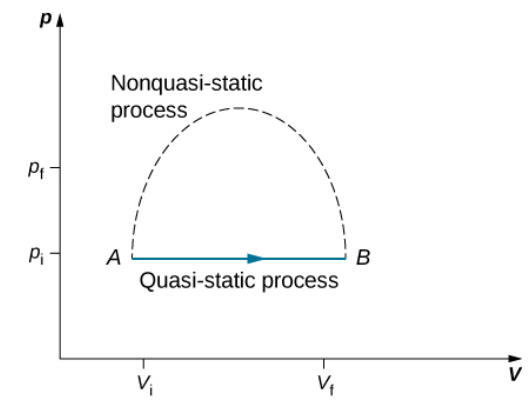
\includegraphics[width=0.5\textwidth]{figures/process.png}
\caption{\label{fig:process} Two processes: quasi-static and non-quasi-static.  We study state transitions composed of many quasi-static transitions.  The pictured non-quasi-static transition has two volumes with the same pressure, so how can we reasonably define the state of a system?}
\end{figure} 
\end{frame}

\begin{frame}{The First Law of Thermodynamics}
Words of the text: ``A quasi-static transition is one in which the change in state is made infinitesimally slowly so that at each instant, the system can be assumed to be at a thermodynamic equilibrium with itself and with the environment.'' \\ \vspace{0.5cm}
\textbf{What follows are a few examples of thermodynamic processes that may be classified as quasi-static.} In realistic systems, some amount of non-quasi-static behavior is normal.
\end{frame}

\begin{frame}{The First Law of Thermodynamics}
A process is called \textbf{cyclic} if it returns a system to the same state with the same internal energy.
We should know at least these types of quasi-static processes: \small 
\begin{enumerate}
\item \alert{Isothermal} ($T$ is constant)
\item Isobaric ($p$ is constant)
\item Adiabatic ($Q$, the head added/subtracted, is zero)
\item Isochoric ($V$ is constant)
\end{enumerate}
Exercise: use the following simulation to create cyclic processes.
\url{https://www.geogebra.org/m/mXvUPjFz}
\end{frame}

\begin{frame}{The First Law of Thermodynamics}
\small
Exercise: use the following simulation to create cyclic processes: \url{https://www.geogebra.org/m/mXvUPjFz}.  What do you notice about the total heat exchanged $Q$, and the total work done, $W$?
\begin{enumerate}
\item Create three processes between states A and B: isobaric, isochoric, and adiabatic.  Explain quantitatively why each fits the relevant criterion.  What is true about $Q$ and $W$ for each of these for processes you've created?
\begin{itemize}
\item \textbf{Isobaric}: what is the slope of an isobaric process?
\item \textbf{Isobaric}: how do you calculate the work done?
\item \textbf{Isochoric}: what is the slope of an isochoric process?
\item \textbf{Isochoric}: what is true of the heat added/subtracted to/from the system?
\item \textbf{Adiabatic}: create several process with $dQ \approx 0$. Calculate $pV^{\frac{5}{3}}$ for each.  What do you notice?
\end{itemize}
\end{enumerate}
\end{frame}

\begin{frame}{The First Law of Thermodynamics}
\small
Exercise: use the following simulation to create cyclic processes: \url{https://www.geogebra.org/m/mXvUPjFz}.  What do you notice about the total heat exchanged $Q$, and the total work done, $W$?
\begin{enumerate}
\item Create three processes between states A and B: isobaric, isochoric, and adiabatic.  Explain quantitatively why each fits the relevant criterion.  What is true about $Q$ and $W$ for each of these for processes you've created?
\item \alert{Consider three different cyclic processes ABCD, and predict the net work done.  Compare your calculations to the simulation output.}
\end{enumerate}
\end{frame}

\section{Heat Capacities of an Ideal Gas}

\begin{frame}{Heat Capacities of an Ideal Gas}
\small What follows is a traditional proof of the following theorem:
\begin{equation}
C_{\rm P} = C_{\rm V} + R
\end{equation}
\textit{The molar heat capacity of a gas at constant pressure is always larger than at constant volume.} \\ \vspace{0.5cm}
\begin{itemize}
\item \textbf{Assume} an ideal gas
\item \textbf{Apply} First Law of Thermodynamics
\item Evidence for \textit{independence of state function}
\item Evidence for \textit{kinetic theory of gases}
\end{itemize}
\end{frame}

\begin{frame}{Heat Capacities of an Idea Gas}
\small
The first law of thermodynamics: $dE = dQ - dW$.  Consider an ideal gas, in a vessel with fixed volume.  Since $dW = pdV$, $dW=0$.  If heat $dQ$ is added to that vessel, the corresponding temperature in increase is
\begin{equation}
dQ = n C_{\rm V} dT
\end{equation}
where $C_{\rm V}$ represents the \textit{heat capacity at constant volume} \footnote{Recall that from kinetic theory, for ideal gases with no molecular interactions, $C_{\rm V} = \frac{3}{2}R$.}.  Because $dE = dQ$,
\begin{equation}
dE = n C_{\rm V} dT
\end{equation}
\end{frame}

\begin{frame}{Heat Capacities of an Idea Gas}
\small
Consider the same gas, but at fixed pressure.  Beginning with the first law of thermodynamics: \\ $dE = dQ - dW = dQ - pdV$.  If heat $dQ$ is added to the vessel, the corresponding temperature change is
\begin{equation}
dQ = n C_{\rm P} dT \label{eq:dq}
\end{equation}
where $C_{\rm P}$ is the \textit{heat capacity at constant pressure.}  In order to obtain an expression for $dE$ involving only temperature, the ideal gas law must be differentiated:
\begin{align}
d(pV) &= d(nRT) \\
pdV &= nRdT \label{eq:pdv}
\end{align}
Substituting the right-hand side of Eq. \ref{eq:pdv} for $dW$ in the First Law, and the right-hand side of Eq. \ref{eq:dq} for $dQ$ in the first law, the result is
\begin{equation}
dE = n(C_{\rm P} - R)dT
\end{equation}
\end{frame}

\begin{frame}{Heat Capacities of an Idea Gas}
The expressions for $dE$ under isobaric and isochoric conditions have been obtained:
\begin{align}
dE &= C_{\rm V} dT \\
dE &= n(C_{\rm P} - R)dT
\end{align}
If the internal energy of a thermodynamic system depends only on the temperature, then these two expressions must be equal.  Upon setting them equal, a fundamental relationship is revealed:
\begin{equation}
\boxed{
C_{\rm P} = C_{\rm V} + R}
\end{equation}
It has been shown that $C_{\rm V} = \frac{3}{2}R$ from the equipartition principle, so $C_{\rm P} = \frac{5}{2}R$ for an ideal gas.
\end{frame}

\begin{frame}{Heat Capacities of an Ideal Gas}
Suppose a cylinder of 1 mole of an ideal gas at fixed pressure is heated for 6 minutes with 10 W of power.  What is the change in temperature?  ($R = 8.314$ J/mol/Kelvin).
\begin{itemize}
\item A: About 20 degrees Kelvin
\item B: About 70 degrees Kelvin
\item C: About 120 degrees Kelvin
\item D: About 170 degrees Kelvin
\end{itemize}
\end{frame}

\section{Adiabatic Processes with an Ideal Gas}

\begin{frame}{Adiabatic Processes with an Ideal Gas}
\textbf{\alert{Adiabatic}} describes a process in which no heat is exchanged, $dQ = 0$.  From the first law of thermodynamics,
\begin{equation}
dE_{\rm int} = -dW
\end{equation}
\textit{Free expansion} is used in the text to refer to the special adiabatic case in which $dW = 0$, so $E_{\rm f,int} = E_{\rm i,int}$.  More interesting is to consider the two forms of heat capacity, of the previous section, corresponding to isobaric and isochoric processes.
\end{frame}

\begin{frame}{Adiabatic Processes with an Ideal Gas}
\small What follows is a traditional proof of the following theorem: \\ \vspace{0.5cm}
Let $\gamma = \frac{C_{\rm P}}{C_{\rm V}}$.  During an adiabatic process, the following quantity remains constant:
\begin{equation}
pV^{\gamma} = const
\end{equation}
\textit{The produce of the pressure and volume to a fixed power remains constant during an adiabatic process.} \\ \vspace{0.5cm}
\begin{itemize}
\item \textbf{Assume} an ideal gas
\item \textbf{Apply} First Law of Thermodynamics
\item Evidence for \textit{independence of state function}
\item Evidence for \textit{kinetic theory of gases}
\end{itemize}
\end{frame}

\begin{frame}{Adiabatic Processes with an Ideal Gas}
Consider an \textit{adiabatic} process ($dQ=0$) in which the First Law of Thermodynamics becomes
\begin{equation}
dE_{\rm int} = -dW = -pdV
\end{equation}
For any ideal gas, the internal energy is proportional to the temperature, regardless of the process type.  Thus,
\begin{equation}
dE_{\rm int} = n C_{\rm V} dT
\end{equation}
Substituting into the First Law and rearranging,
\begin{equation}
dT = -\frac{pdV}{n c_{\rm V}} \label{eq:t1}
\end{equation}
\end{frame}

\begin{frame}{Adiabatic Processes with an Ideal Gas}
\small
As before, differentiating the the idea gas law, assuming both pressure and volume may vary, yields
\begin{equation}
dT = \frac{dp V+pdV}{nR} \label{eq:t2}
\end{equation}
Equating these two expressions for $dT$, Eq. \ref{eq:t1} and Eq. \ref{eq:t2}, gives 
\begin{equation}
C_{\rm V} V dp + \left( C_{\rm V} + R \right) p dV = 0 \label{eq:almost}
\end{equation}
Recall that $C_{\rm V} + R = C_{\rm p}$.  Using this, Eq. \ref{eq:almost} becomes
\begin{equation}
C_{\rm V} V dp + C_{\rm p} p dV = 0 \label{eq:almost2}
\end{equation}
Letting $\gamma = \frac{C_{\rm p}}{C_{\rm V}} > 1$, Eq. \ref{eq:almost2} reads
\begin{equation}
V dp + \gamma p dV = 0 \label{eq:gamma}
\end{equation}
\end{frame}

\begin{frame}{Adiabatic Processes with an Ideal Gas}
Rearranging Eq. \ref{eq:gamma} and integrating both sides,
\begin{align}
\int \frac{dp}{p} + \gamma \int \frac{dV}{V} &= 0 \\
\ln p + \ln V^{\gamma} &= const \\
\ln pV^{\gamma} &= const \\
pV^\gamma &= const
\end{align}
Thus, the theorem holds:
\begin{equation}
\boxed{ pV^\gamma = const}
\end{equation}
\end{frame}

\begin{frame}{Adiabatic Processes with an Ideal Gas}
The reason this result is important is now we have a way to describe adiabatic transitions on $pV$ diagrams.
\begin{figure}
\centering
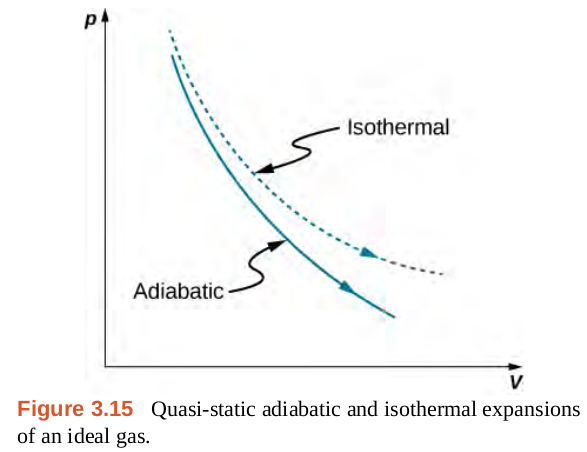
\includegraphics[width=0.6\textwidth]{figures/adiabatic.png}
\caption{\label{fig:adiabatic} Isothermal: $pV = const$.  Adiabatic: $pV^\gamma = const$.}
\end{figure}
\end{frame}

\begin{frame}{Adiabatic Processes with an Ideal Gas}
\small
With an understanding of $pV$ behavior of different processes, and the First Law, we can begin to construct more complex processes, and predict the work done, and heat required.
\begin{figure}
\centering
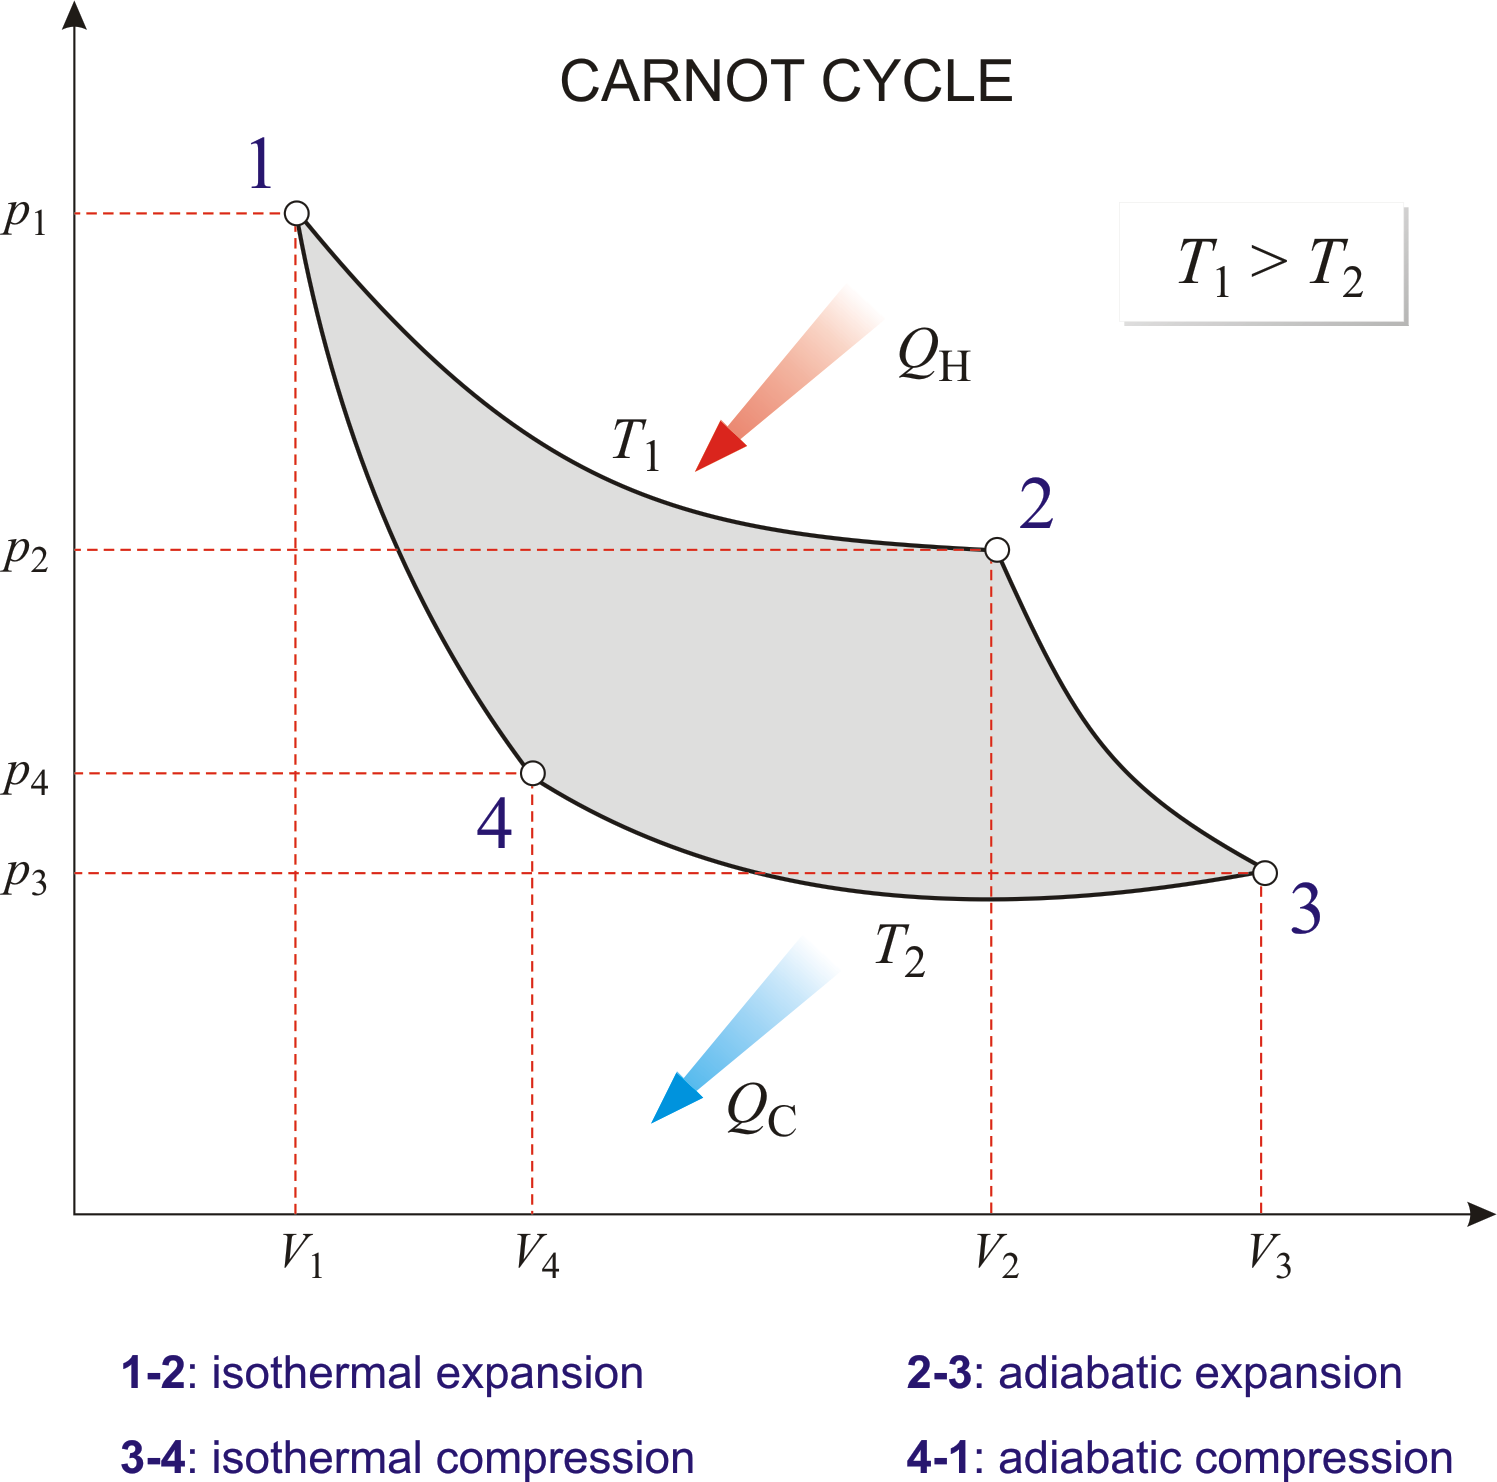
\includegraphics[width=0.5\textwidth]{figures/carnot_cycle.png}
\caption{\label{fig:carnot} An example of a complex cycle: the Carnot cycle.}
\end{figure}
\end{frame}

\begin{frame}{Adiabatic Processes with an Ideal Gas}
We have seen how \textbf{cyclic} processes have $dE_{\rm int} = 0$, so $dQ = dW$ by the First Law.  However, we need to introduce \textit{how} to calculate the $dQ$ to perform a given process, so that we may know the predicted work to be done. \\ \vspace{0.5cm}
\textit{Isothermal process, ideal gas}:
\begin{align}
dW &= pdV \\
dW &= \frac{nRT dV}{V} \\
\int dW &= \int \frac{nRT dV}{V} \\
W &= nRT \ln\left(\frac{V_{\rm f}}{V_{\rm i}}\right)
\end{align}
\end{frame}

\begin{frame}{Adiabatic Processes with an Ideal Gas}
Heat required to change the volume of an idea gas isothermically:
\begin{equation}
\boxed{Q = nRT \ln\left(\frac{V_{\rm f}}{V_{\rm i}}\right)} \label{eq:isoT}
\end{equation}
We can repeat this procedure for adiabatic processes:
\begin{equation}
\boxed{W = \frac{1}{1-\gamma}\left(p_{\rm f}V_{\rm f} - p_{\rm i}V_{\rm i}\right)} \label{eq:ad}
\end{equation}
In Eq. \ref{eq:ad}, $k = p_{\rm i}V_{\rm i}^\gamma = p_{\rm f}V_{\rm f}^\gamma$.  The utility of these formulae: \alert{we can predict the heat required to go from one known state to another}.  The isobaric and isochoric processes are much simpler, but the derivation is similar.
\end{frame}

\begin{frame}{Adiabatic Processes with an Ideal Gas}
\small 
\textbf{Example 3.7 from Section 3.6 of text}.  Gasoline vapor is injected into the cylinder of an automobile engine when the piston is in its expanded position.
The temperature, pressure, and volume of the resulting gas-air mixture are 20 deg C, $10^5$ Pa, and 240 cm$^3$.  The mixture is then compressed adiabatically to a volume of 40 cm$^3$.  (a) What are the pressure and temperature of the mixture after the compression? (b) How much work is done by the mixture during the compression?
\begin{itemize}
\item Part (a), example.
\item Part (b), \textbf{groups on board.}
\end{itemize}
\end{frame}

\begin{frame}{Adiabatic Processes with an Ideal Gas}
\begin{figure}
\centering
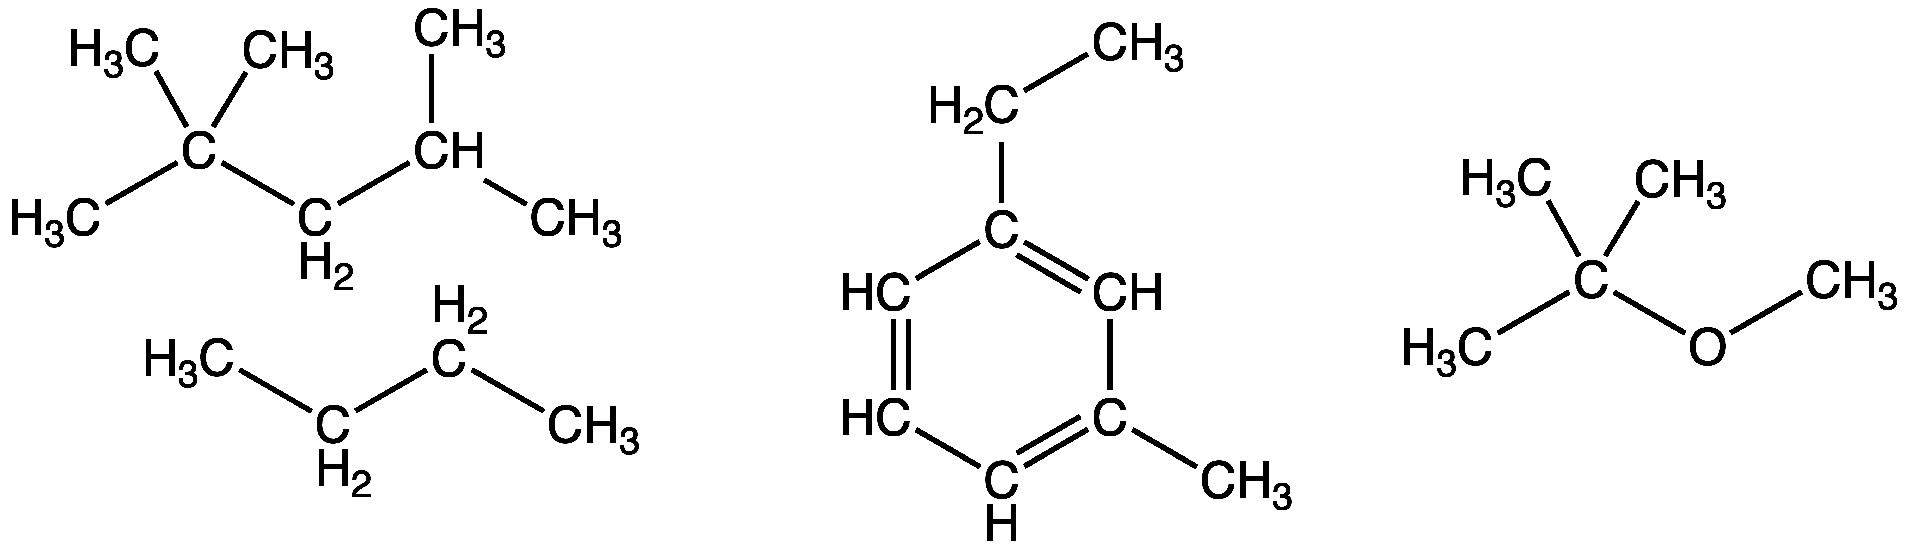
\includegraphics[width=0.85\textwidth]{figures/GasolineComp.png}
\caption{\label{fig:gas} Gasoline components are polyatomic. From left to right: isooctane, butane, 3-ethyltoluene, and MTBE.}
\end{figure}
\end{frame}

\begin{frame}{Adiabatic Processes with an Ideal Gas}
One mole of an ideal gas ($d=5$) in a piston is at a temperature of 600 K, a pressure of 2 atm, and a volume of 1.0 L.  How much work is done if the volume expands  \alert{isothermically} by a factor of 2.718?
\textbf{Group exercise on board.}
\end{frame}

\begin{frame}{Adiabatic Processes with an Ideal Gas}
One mole of an ideal gas ($d=5$) in a piston is at a temperature of 600 K, a pressure of 2 atm, and a volume of 1.0 L.  How much work is done if the volume expands  \alert{adiabatically} by a factor of 2.718?
\textbf{Group exercise on board.}
\end{frame}

\section{The Second Law of Thermodynamics}

\begin{frame}{The Second Law of Thermodynamics}
\textit{The First Law of Thermodynamics} states that
\begin{equation}
dE_{\rm int} = dQ - dW
\end{equation}
Pause for a moment and think intuitively: is \textit{all} of the change in internal energy of a system is \textit{exactly all} of the \textbf{heat added} minus the the work done by the system? \\ \vspace{0.5cm}
Actually, yes, this is not an approximation, for energy must be conserved (Newton's laws). \\ \vspace{0.5cm}
\alert{The Second Law of Thermodynamics} addresses \textbf{where} the heat is, and how \textbf{efficiently} it becomes work.
\end{frame}

\begin{frame}{The Second Law of Thermodynamics}
\small
The key to understanding the \alert{Second Law of Thermodynamics} is the \textbf{reversability} of a process.  A simulation to demonstrate this:
\url{https://phet.colorado.edu/en/simulation/reversible-reactions} \\ \vspace{0.5cm}
Assignment for this activity:
\begin{enumerate}
\item Learn the controls: barrier, adding particles, and adding heat.
\item Raise the barrier, and add a few particles to one chamber.  Increase the temperature, and lower the barrier.  How long does it take for the system to equilibrate, and how does this depend on temperature?
\item Can you raise the barrier, trapping all particles on one side?
\item Repeat with an \textbf{increasingly large number of particles.}  What are the results?
\end{enumerate}
\end{frame}

\begin{frame}{The Second Law of Thermodynamics}
\small
\begin{enumerate}
\item Learn the controls: barrier, adding particles, and adding heat.
\item Raise the barrier, and add a few particles to one chamber.  Increase the temperature, and lower the barrier.  How long does it take for the system to equilibrate, and how does this depend on temperature?
\item Can you raise the barrier, trapping all particles on one side?
\item Repeat with an \textbf{increasingly large number of particles.}  What are the results?
\item \textbf{Group discussion at the conclusion.}  How do the results depend on temperature?  Is energy of the initial state conserved?
\end{enumerate}
\end{frame}

\begin{frame}{The Second Law of Thermodynamics}
\small
Some vocabulary words:
\begin{itemize}
\item \textbf{Quasi-static}: describes a process during which the system is at each step in equilibrium with the surroundings
\item \textbf{Reversible}: decribes a process in which the state of a system changes but the system can be returned to the original state.  Required to be quasi-static.
\item \textbf{Irreversible or natural}: describes a process in which a system cannot be restored perfectly to the original state.
\item \textbf{Isobaric}: constant pressure ($W=p\Delta V$).  In theory, reversible.
\item \textbf{Isochoric}: constant volume ($W=0$).  In theory, reversible.
\item \textbf{Isothermal}: constant temperature ($\Delta T = 0$, $p \propto V^{-1}$).  In theory, reversible.
\item \textbf{Adiabatic}: $\Delta Q = 0$.  In theory, reversible.
\end{itemize}
\end{frame}

\section{JITT 1.4}

\begin{frame}{JITT 1.4}
\begin{enumerate}
\item How many statements of the Second Law of Thermodynamics are there?  What do they mean, in general?
\item What is the efficiency of a Carnot cycle when the temperature of the input ($T_h$) is four times as large as the temperature of the output ($T_c$)? 
\item If a process is cyclic, does this imply that the entropy is constant?  What conditions are necessary for this?
\end{enumerate}
\end{frame}

\begin{frame}{JITT 1.4}
\textbf{How many statements of the Second Law of Thermodynamics are there?  What do they mean, in general?} \\ \vspace{0.5cm}
``There are three statements of the second law of thermodynamics. The statements are Clausius, entropy, and Kelvin.''
\begin{itemize}
\item heat will never flow from a cold object to a hot one
\item entropy never decreases
\item it is impossible to turn heat into work without any other effects
\item no engine working between two reservoirs at constant temperature can have the greater efficiency than a reversible engine
\end{itemize}
\end{frame}

\begin{frame}{JITT 1.4}
\textbf{What is the efficiency of a Carnot cycle when the temperature of the input ($T_h$) is four times as large as the temperature of the output ($T_c$)?} \\ \vspace{0.5cm}
``The efficiency can be calculated by the following formula:''
\begin{equation}
e = 1 - \frac{T_c}{T_h} = 1 - \frac{1}{4} = \frac{3}{4}
\end{equation}
\end{frame}

\begin{frame}{JITT 1.4}
\textbf{If a process is cyclic, does this imply that the entropy is constant?  What conditions are necessary for this?} \\ \vspace{0.5cm}
``The entropy is zero if it is cyclic." \\
``yes, the temperature and heat must return to same values.'' \\
``The entropy is only constant when the process is reversible.''
\end{frame}

\begin{frame}{The Second Law of Thermodynamics}
\begin{tcolorbox}[colback=white,colframe=red!40!blue,title=The \textit{Clausius Statement} of the Second Law of Thermodynamics]
\alert{Heat never flows spontaneously from a colder object to a hotter object.}
\end{tcolorbox}
\end{frame}

\begin{frame}{The Second Law of Thermodynamics}
Another subject that guides us to think about The Second Law of Thermodynamics is \textit{heat engines}.
\begin{figure}
\centering
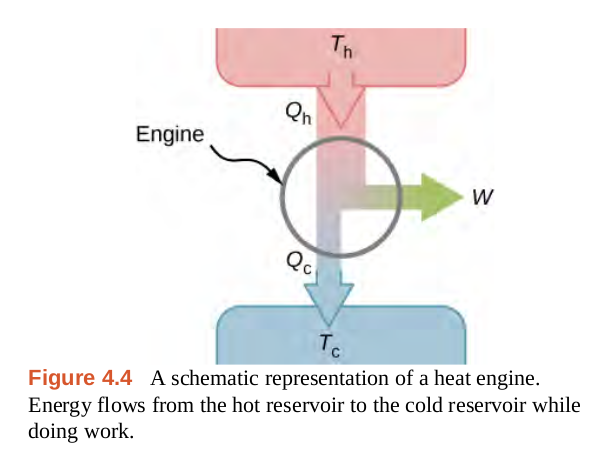
\includegraphics[width=0.55\textwidth]{figures/engine.png}
\caption{\label{fig:engine} A canonical engine.  Every engine involving heat follows this general pattern.  Let the engine undergo a cyclic process, $\Delta E_{\rm int} = 0$, and $Q = Q_{\rm h} - Q_{\rm c}$.}
\end{figure}
\end{frame}

\begin{frame}{The Second Law of Thermodynamics}
From The First Law of Thermodynamics:
\begin{align}
dE_{\rm int} &= Q - W \\
0 &= Q_{\rm h} - Q_{\rm c} - W \\
W &= Q_{\rm h} - Q_{\rm c}
\end{align}
So the work performed by an engine is
\begin{equation}
\boxed{W = Q_{\rm h} - Q_{\rm c}}
\end{equation}
$Q_{\rm h}$ is like the heat input, the fuel, and $Q_{\rm c}$ is the exhaust or discarded heat.  The \textit{efficiency} is the work done for the fuel burned: $e = \frac{W}{Q_{\rm h}}$.
\end{frame}

\begin{frame}{The Second Law of Thermodynamics}
Efficiency of a general heat engine:
\begin{equation}
\boxed{
e = \frac{W}{Q_{\rm h}} = \frac{Q_{\rm h}-Q_{\rm c}}{Q_{\rm h}} = 1-\frac{Q_{\rm h}}{Q_{\rm c}}
}
\end{equation}
\end{frame}

\begin{frame}{The Second Law of Thermodynamics}
Another subject that guides us to think about The Second Law of Thermodynamics is \textit{refridgeration}.
\begin{figure}
\centering
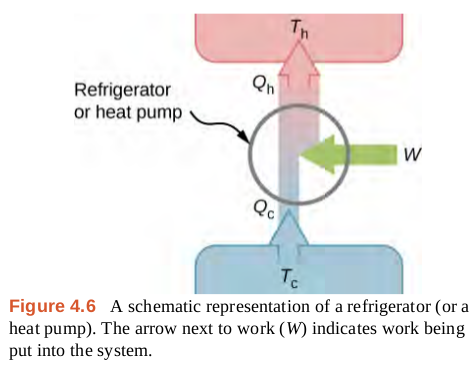
\includegraphics[width=0.55\textwidth]{figures/fridge.png}
\caption{\label{fig:fridge} A canonical refridgerator.  All refridgeration follows this general pattern.  Let the engine undergo a cyclic process, $\Delta E_{\rm int} = 0$, and $Q = Q_{\rm h} - Q_{\rm c}$.}
\end{figure}
\end{frame}

\begin{frame}{The Second Law of Thermodynamics}
By the way, the refridgeration diagram also applies to \textit{heat pumps}, where work is done on cold air to make it warmer, and then it is released into a warmer environment.  Two more equations:
\begin{equation}
K_{\rm R} = \frac{Q_{\rm c}}{W} = \frac{Q_{\rm c}}{Q_{\rm h}-Q_{\rm c}}
\end{equation}
The coefficient of performance for refridgeration, $K_{\rm R}$.
\begin{equation}
K_{\rm P} = \frac{Q_{\rm h}}{W} = \frac{Q_{\rm h}}{Q_{\rm h}-Q_{\rm c}}
\end{equation}
The coefficient of performance for a heat pump, $K_{\rm P}$.  $K_{\rm P} = 1/e$.
\end{frame}

\begin{frame}{The Second Law of Thermodynamics}
What is the largest value $e$ can theoretically take?
\begin{itemize}
\item A: 0.0
\item B: Approaching 1.0 but never reaching 1.0
\item C: Exactly 1.0
\item D: I am confused.
\end{itemize}
\end{frame}

\begin{frame}{The Second Law of Thermodynamics}
Suppose we have a rudimentary engine that extracts energy from the motions of a finite number of molecules.  What is required for an efficiency $e=1.0$?
\begin{itemize}
\item A: To extract energy so well that all the molecules stop moving.
\item B: To extract energy so well that all the molecules almost stop moving, but still move a little.
\item C: To extract energy so well that some of the molecules are stationary, but some still move.
\item D: I am confused.
\end{itemize}
\end{frame}

\begin{frame}{The Second Law of Thermodynamics}
Choosing from the reasons below, what is the reason that it is ``not possible'' to extract energy so well we have $e=1.0$?
\begin{itemize}
\item A: There are no instruments that precise, that can select individual molecules.
\item B: Molecules have some un-extractable amount of energy.
\item C: There's an enormous number of ways molecules can have energy, and a small number of ways they can have none.
\item D: I am confused.
\end{itemize}
\end{frame}

\begin{frame}{The Second Law of Thermodynamics}
What is the highest possible number the coefficient of performance $K_{\rm R}$ for refridgeration can take?  (Think of the formula, but also think \textit{conceptually}.  How is this number defined?).
\begin{itemize}
\item A: 0
\item B: 1
\item C: Infinity
\item D: I am confused.
\end{itemize}
\end{frame}

\begin{frame}{The Second Law of Thermodynamics}
\begin{tcolorbox}[colback=white,colframe=red!40!blue,title=The \textit{Kelvin Statement} of the Second Law of Thermodynamics]
\alert{It is impossible to convert the heat from a single source into work without any other effect.}
\end{tcolorbox}
\textit{Corollary:} It is impossible to construct a heat engine with $e=1.0$.  There are many proofs and examples in the reading.
\end{frame}

\begin{frame}{The Second Law of Thermodynamics}
\begin{figure}
\centering
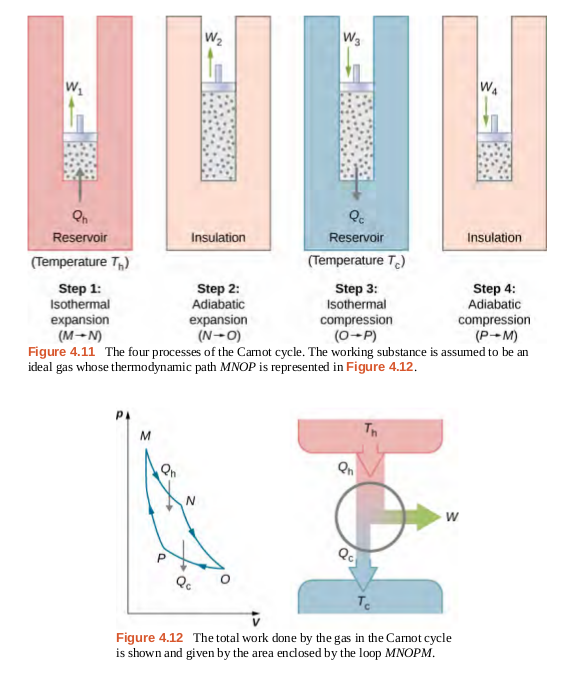
\includegraphics[width=0.5\textwidth]{figures/carnot1.png}
\caption{\label{fig:carnot2} \textbf{The Carnot Cycle}: the most efficient cyclic process between a single hot and cold resevoir.}
\end{figure}
\end{frame}

\begin{frame}{The Second Law of Thermodynamics}
The Carnot Cycle consists of four steps:
\begin{enumerate}
\item Isothermal expansion by adding heat $Q_{\rm h}$
\item Adiabatic expansion, the temperature lowers to $T_{\rm c}$
\item Isothermal compression by removing heat $Q_{\rm c}$
\item Adiabatic compression, the temperature rises to $T_{\rm h}$
\end{enumerate}
Work gained: $W = Q_{\rm h} - Q_{\rm c}$, at an efficiency $e = 1-\frac{Q_{\rm c}}{Q_{\rm h}}$.
\end{frame}

\begin{frame}{The Second Law of Thermodynamics}
Using Eqs. \ref{eq:isoT} and \ref{eq:ad}, and the definition of efficiency ($1-\frac{Q_{\rm c}}{Q_{\rm h}}$), it may be shown that
\begin{equation}
\boxed{
e_{\rm Carnot} = 1 - \frac{T_{\rm c}}{T_{\rm h}}}
\end{equation}
\end{frame}

\begin{frame}{The Second Law of Thermodynamics}
An engine following the 4-stroke Carnot cycle burns fuel at a temperature of 1000 K, and the exhaust is at a temperature of 300 K.  What is the efficiency of this engine?
\begin{itemize}
\item A: 1.0
\item B: 0.5
\item C: 0.7
\item D: 0.9
\end{itemize}
\end{frame}

\begin{frame}{The Second Law of Thermodynamics}
An engine following the 4-stroke Carnot cycle has an efficiency of 0.4 and exhausts heat at a temperature of 300 K.  What is the temperature of the fuel burn?
\begin{itemize}
\item A: 100 K
\item B: 200 K
\item C: 500 K
\item D: 1000 K
\end{itemize}
\end{frame}

\begin{frame}{The Second Law of Thermodynamics}
A vehicle needs to do 3 kJ of work pulling an object up a hill.  The engine follows a Carnot cycle and burns fuel at 1200 K with exhaust at 300 K.  How much heat is required to put into that engine to accomplish the work?
\begin{itemize}
\item A: 3 kJ
\item B: 4 kJ
\item C: 5 kJ
\item D: 6 kJ
\end{itemize}
\end{frame}

\begin{frame}{The Second Law of Thermodynamics}
Final concept: \textbf{Entropy}.  Let the change in \textit{entropy} $S$, which is a path-independent state function like energy, be defined by
\begin{equation}
\Delta S = \int_{A}^B \frac{dQ}{T}
\end{equation}
For ideal quasi-state reversible processes,
\begin{equation}
\Delta S = \oint \frac{dQ}{T} = 0
\end{equation}
What are the units of entropy?  \textbf{Final problem:} show that Boltsmann's constant, $k_{\rm B}$ has units of entropy. (Group exercise).
\end{frame}

\begin{frame}{The Second Law of Thermodynamics}
The final statement of the Second Law of Thermodynamics summarizes Carnot engines, the Kelvin and Clausius statements:
\\ \vspace{0.5cm}
\begin{tcolorbox}[colback=white,colframe=red!40!blue,title=The \textit{Entropy Statement} of the Second Law of Thermodynamics]
\alert{$\Delta S \geq 0$ for any natural process.}
\end{tcolorbox}
\vspace{0.5cm}
\textit{Think about the Carnot cycle, and how it has the smallest possible entropy gain.}
\end{frame}

\begin{frame}{The Second Law of Thermodynamics}
\begin{figure}
\centering
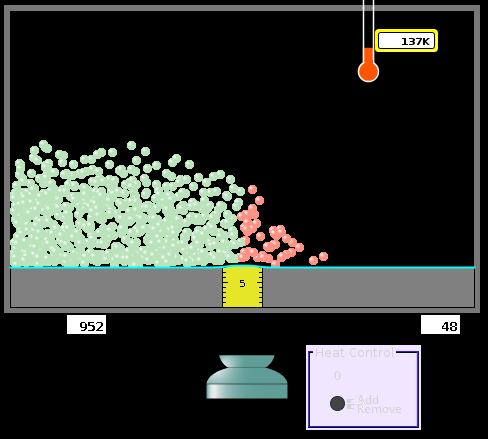
\includegraphics[width=0.4\textwidth]{figures/S1.png}
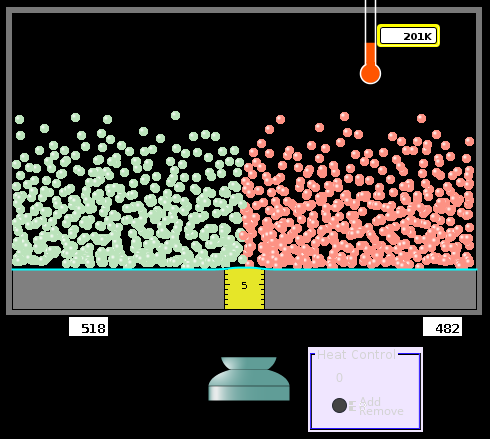
\includegraphics[width=0.4\textwidth]{figures/S2.png}
\caption{\label{fig:s} (Left) Low entropy, $S_{\rm 1}$.  (Right) High entropy, $S_{\rm 2} \gg S_{\rm 1}$.}
\end{figure}
\end{frame}

\begin{frame}{The Second Law of Thermodynamics}
\textit{Potential paper topic: history of the scientific development of the steam power plant.}
\end{frame}

\section{Conclusion}

\begin{frame}{Unit 2 Summary}
\textbf{Reading: Chapters 3 and 4}
\begin{enumerate}
\item The First Law of Thermodynamics
\begin{itemize}
\item $dE = dQ - dW$
\item Sign conventions
\item State variables and path independence, $pV$ diagrams
\item Cyclic processes
\item Heat capacities and the First Law
\item Isothermal and adiabatic processes
\end{itemize}
\item The Second Law of Thermodynamics
\begin{itemize}
\item Probabilistic notions of entropy
\item Clausius statement
\item Kelvin statement
\item Carnot cycle
\item Formal definition of entropy
\end{itemize}
\end{enumerate}
\end{frame}

\section{Answers}

\begin{frame}{Answers}
\tiny
\begin{columns}[T]
\begin{column}{0.5\textwidth}
\begin{itemize}
\item 420 seconds
\item Several hours (approx. 12 hours)
\item The extensive variables are $V$ and $n$, and $p$, and $T$ are the intensive ones
\item $E_{\rm int}$ decreases
\item $E_{\rm int}$ does not change
\item $E_{\rm int}$ increases
\item $E_{\rm int}$ decreases
\item $E_{\rm int}$ increases
\item Path 5 most work, path 2 least work.
\item AB: path 2, BA: returns along path 5
\item Path 5
\item 3460 J
\item 2305 J
\item -2305 J
\item 50 J
\item 2 degrees C
\item 0.2 degrees C
\item Fill an inflatable object with heated air at high pressure.
\item About 170 degrees Kelvin
\end{itemize}
\end{column}
\begin{column}{0.5\textwidth}
\begin{itemize}
\item Approaching 1.0 but never reaching 1.0, if it is a natural process
\item To extract energy so well that all the molecules stop moving.
\item There's an enormous number of ways molecules can have energy, and a small number of ways they can have none.
\item Infinity
\item 0.7
\item 500 K
\item 4 kJ
\end{itemize}
\end{column}
\end{columns}
\end{frame}

\end{document}
